\documentclass{scrartcl}

\usepackage[utf8]{inputenc}   % accents
\usepackage[T1]{fontenc}      % caractères français
\usepackage{geometry}         % marges
\usepackage[francais]{babel}  % langue
\usepackage{graphicx}         % images
\usepackage{verbatim}
\usepackage{url}
\usepackage{listings}
\lstset{
  literate=%
    {ê}{{\'e}}1
    {é}{{\'e}}1
    {è}{{\'e}}1
}
\usepackage{float}
\bibliographystyle{alpha}

\title{Apprendre et comprendre l'improvisation musicale}
\subtitle{Mémoire}
\author{Alexandre Casanova--Franger\\
  \and
  Gauthier Lamarque\\
  \and
  Paul Simorre\\
  \and
  Lucas Vivas\\}

\begin{document}

\maketitle
\newpage
\tableofcontents
\newpage


\section{Introduction}
\paragraph{}
Ce projet a été réalisé par quatre étudiants de première année de
Master Informatique de l'Université de Bordeaux (parcours Génie
Logiciel), dans le cadre de l'UE Projet de Programmation.

\subsection{Un outil pour assister l'improvisation musicale}
\paragraph{}
Le projet a été proposé par Myriam Desainte-Catherine, chercheur au
Studio de Création et de Recherche en Informatique et Musiques
Expérimentales (SCRIME) et enseignante à l'ENSEIRB-MATMECA, et Yacine
Amarouchene, physicien du Laboratoire d'Onde et Matière d'Aquitaine
(LOMA). Il a été pensé comme un outil d'aide à "l'improvisation
musicale", un dispositif permettant d'aider un groupe de musiciens à
improviser mais permettant aussi de mieux comprendre la nature de
l'improvisation en musique.

\subsection{Improvisation et corrélation}
\paragraph{}

Il est essentiel de comprendre ces deux notions afin de bien situer
l'intérêt du projet.

\paragraph{}
Lors d'une improvisation en groupe, des musiciens jouent sans règles
établies ; ils cherchent alors à fournir à leur auditoire une
production cohérente, ou du moins au sein de laquelle chaque musicien
joue un rôle dans l'harmonie du morceau en s'accordant avec ses
pairs. La relation qui unit le jeu de deux musiciens et évalue la
qualité de leur accord porte un nom : c'est la corrélation.
\paragraph{}
Au sens premier et basique du terme, la corrélation est le rapport
réciproque entre deux éléments. En statistiques, on parle souvent de
corrélation pour mesurer l'intensité de la liaison existant entre deux
variables.
Dans le cadre de l'étude de signaux sonores, nous faisons le calcul de
corrélation entre deux signaux. Cette corrélation cherche à mesurer
la similarité entre ces deux signaux suivant
différents critères, par exemple la longueur d'onde.
\paragraph{}
En musique, il n'existe pas une mais un nombre indéfini de "fonctions
de corrélation" potentiellement existantes, dont la complexité
varie.
Un exemple de fontion de corrélation assez parlant serait une corrélation
rythmique qui comparerait le tempo de chacun des deux signaux.


% les
% traductions graphiques de ces signaux par transformée de Fourier
% peuvent jouer le rôle des courbes dont on mesure la corrélation. Tout
% au long du déroulement de notre projet, nous travaillons uniquement
% sur des fonctions de corrélation portant sur la comparaison des
% signaux graphiques obtenus à partir des pistes sonores.

% \paragraph{}
% En musique, il n'existe pas une mais un nombre indéfini de "fonctions
% de corrélation" potentiellement existantes, dont la complexité
% varie. "Comprendre" la corrélation et l'improvisation, dans le cadre
% de ce projet, c'est aussi trouver, inventer la fonction de corrélation
% qui répond le mieux aux besoins d'un groupe d'improvisateurs. Une
% bonne fonction de corrélation, dans ce cadre spécifique, est une
% fonction qui fait en sorte qu'un groupe de musiciens joue un morceau
% plus satisfaisant lorsque ses membres sont davantage corrélés.

\subsection{L'existant}
\paragraph{}
Ce projet a été initié par les clients précédemment cités il y a plus
d'un an. Nous sommes le troisième groupe à travailler sur ce projet et
développons donc sur la base des travaux réalisés successivement par
nos prédécesseurs.

\subsubsection{Premiers travaux réalisés sur le projet}
\paragraph{}
Les premiers travaux portant sur ce projet ont été réalisés par un
groupe de six étudiants de l'ENSEIRB-MATMECA. Cette équipe est la
première à réaliser un programme informatique analysant et comparant
des pistes mono-instrumentales pour évaluer leurs corrélations. Ce
programme, prenant en entrées des pistes sonores, retourne une matrice
graphique prenant les mêmes pistes en abscisses et en ordonnées et
retournant pour chaque case une couleur permettant d'évaluer la
corrélation existant entre les deux pistes correspondantes grâce à un
code couleur précis.

\begin{figure}[h]
 \centering
 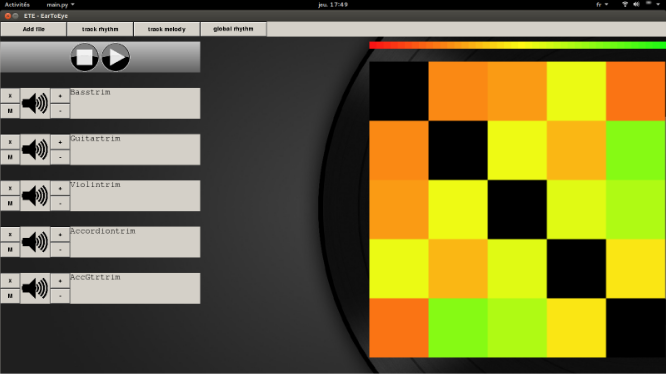
\includegraphics[scale=0.5]{matriceenseirb.png}
 \caption{Capture d'écran du projet mené par les étudiants de l'ENSEIRB}
 \label{matrice-enseirb}
\end{figure}

\paragraph{}
Ci-dessus, la matrice obtenue à l'issue d'un test du programme. Plus
la couleur d'une case est proche du vert, plus la corrélation entre
les deux pistes correspondant au point d'abscisse et au point
d'ordonnée est élevée. À l'inverse, une case dont la couleur est
proche du rouge indique que les deux pistes évaluées sont
décorrélées. La corrélation d'une piste mono-instrumentale avec
elle-même, qui donne toujours un résultat maximal, n'est pas calculée,
ce qui se traduit sur le résultat graphique ci-dessus par une
diagonale de cases noires. La matrice de corrélation est donc
systématiquement symétrique.

\subsubsection{Le système embarqué BELA}
\paragraph{}
Avant de confier la suite du projet à d'autres étudiants, nos clients
ont choisi de changer de support et sont donc passé à un système
embarqué particulier : BELA.\cite{BELA}
% Avant de confier la suite du projet à d'autres étudiants, nos clients
% ont choisi de le rendre plus fonctionnel grâce à l'emploi d'un système
% embarqué particulier : BELA.

\paragraph{}
Ce changement de support est dû au fait que, premièrement ce système est
largement plus portable par rapport à un ordinateur ce qui est un avantage,
mais la raison principale est que BELA est basé sur un système appelé Xenomai Linux, un framework qui ajoute au noyau Linux des éléments permettant de traiter des opérations en temps réel.\cite{XENOMAI}
%link : https://xenomai.org/
%link : https://bela.io/
Cela permet au système de faire du traitement audio en temps réel avec un temps de latence extrêmement faible (100 microsecondes).

\begin{figure}[h]
 \centering
 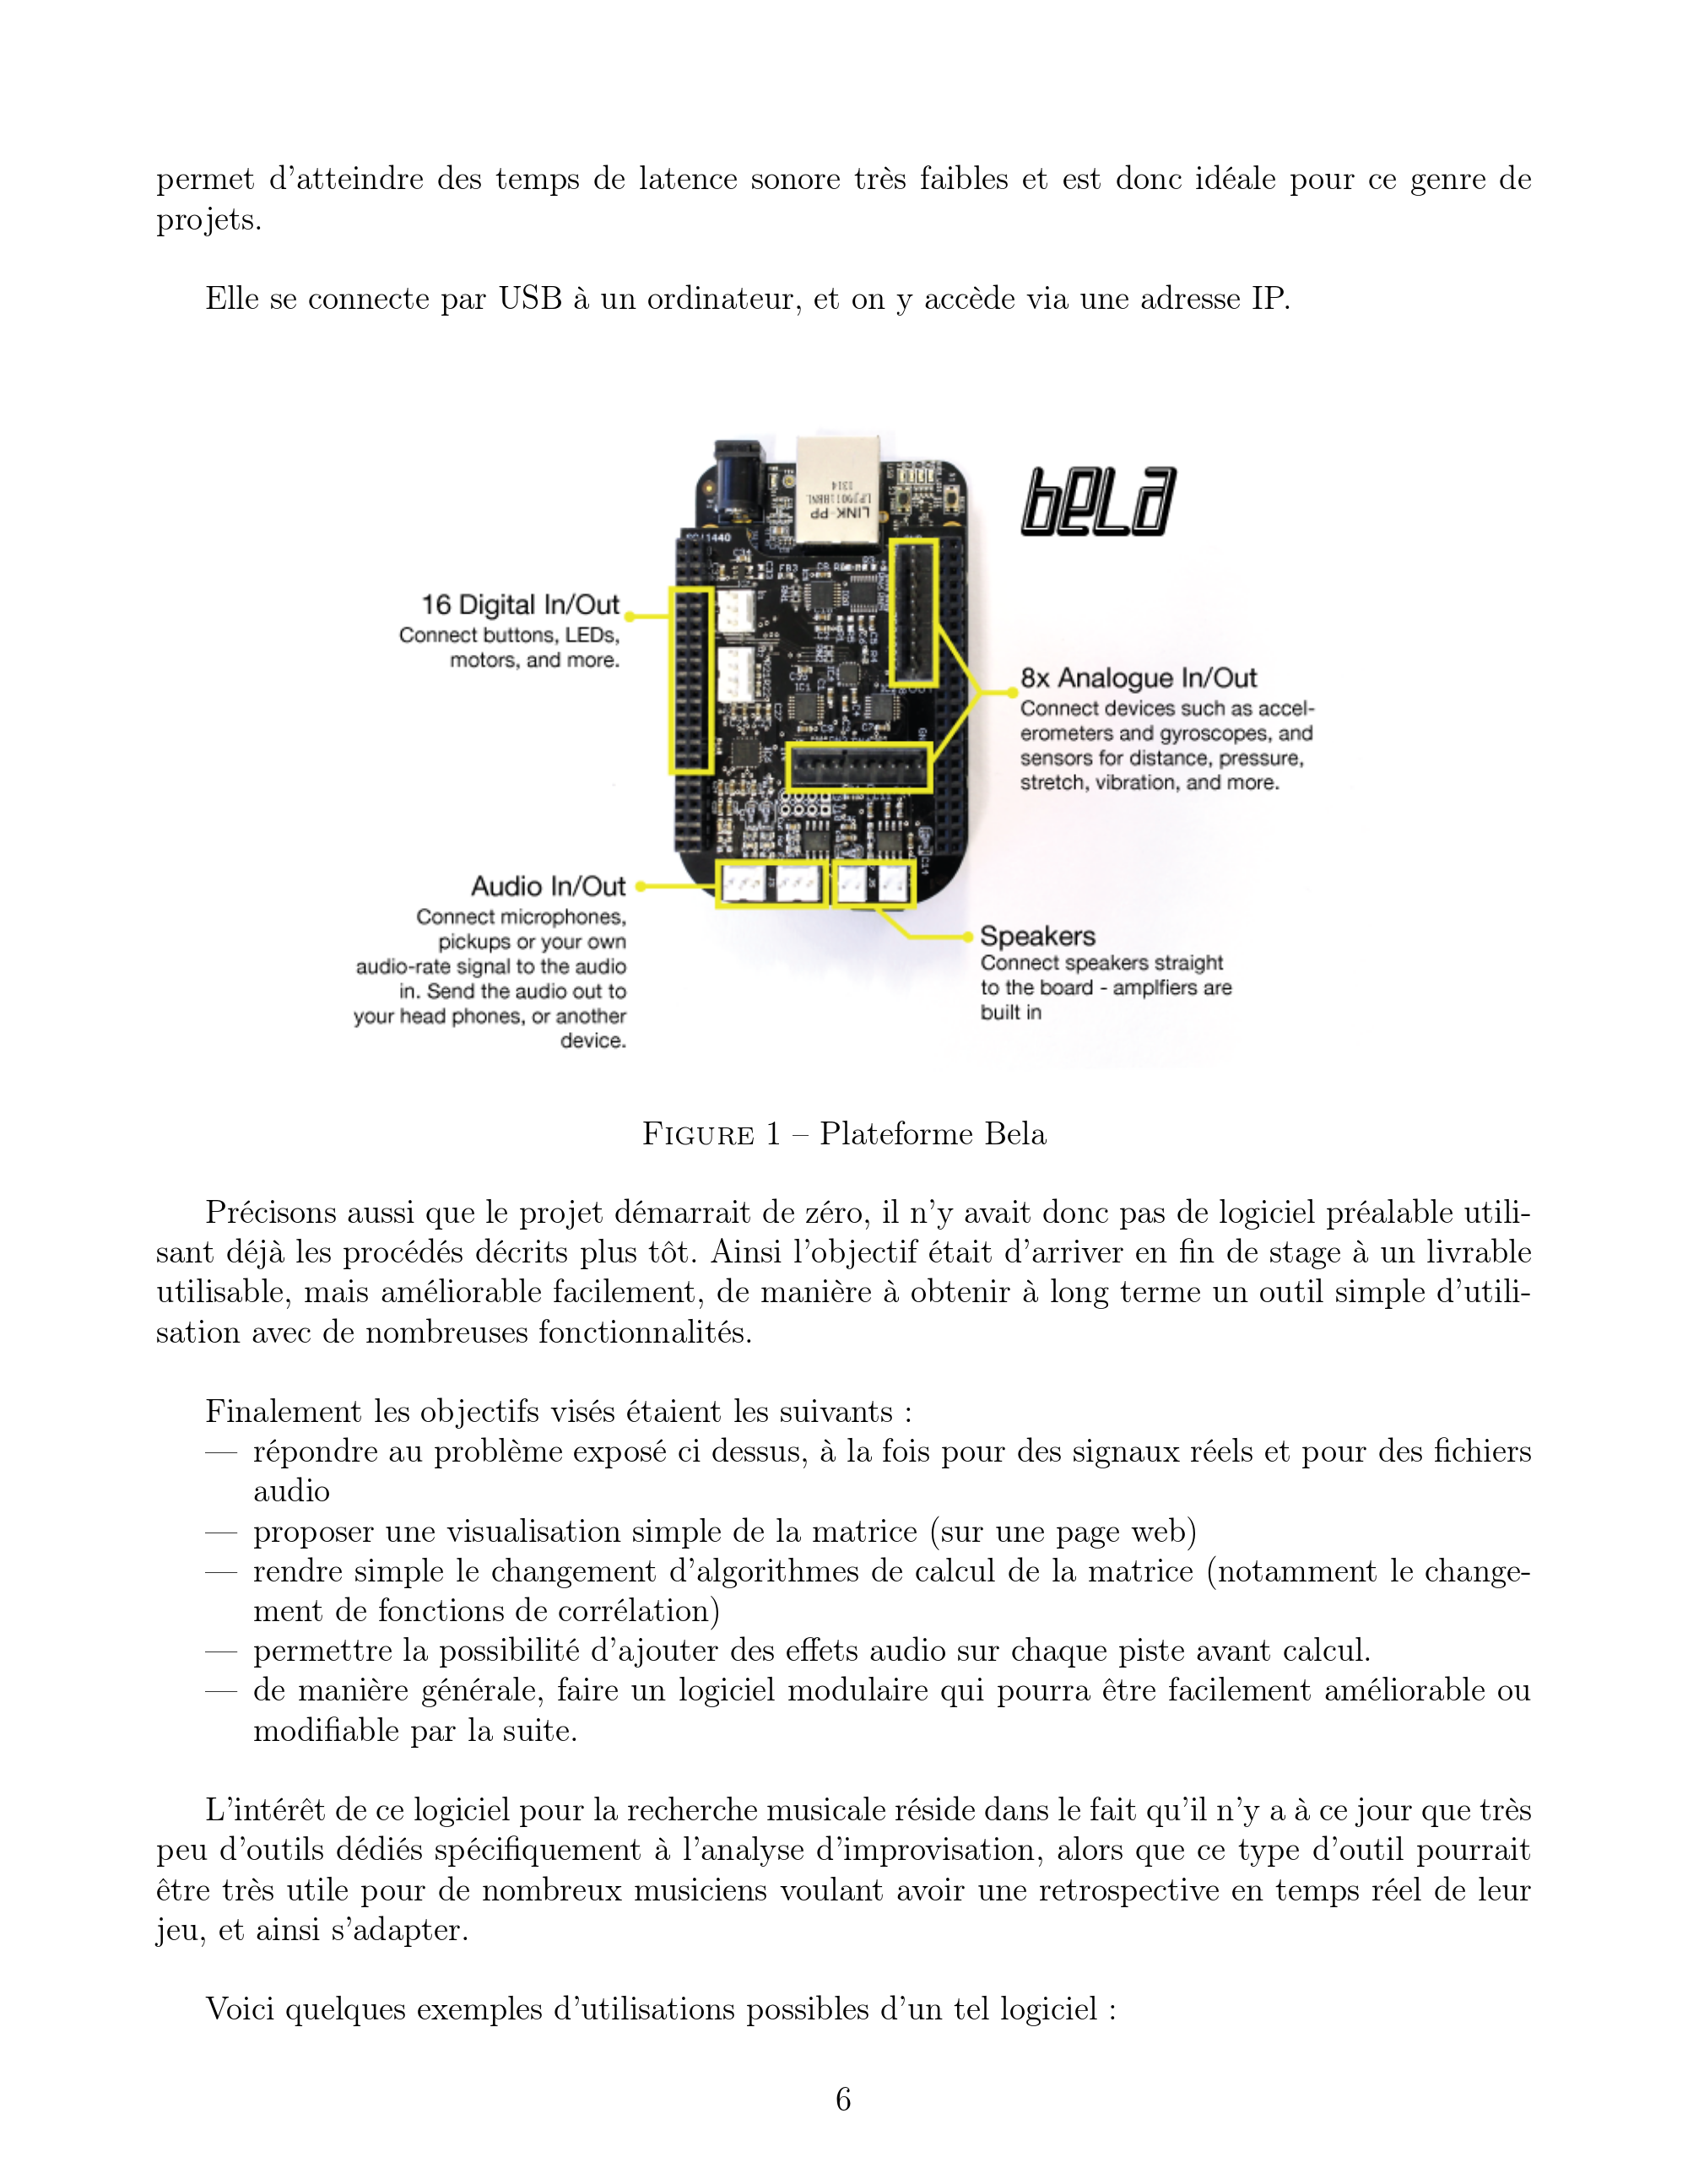
\includegraphics[scale=0.2]{bela.png}
 \caption{Capture de la documentation proposée par le site officiel de Bela}
 \label{bela}
\end{figure}

\paragraph{}
L'aperçu du dispositif externe de BELA présenté ci-dessus témoigne
notamment de la présence d'entrées analogiques pour connecter des
instruments électriques ou enregistreurs sonores. On comprend alors
que le rôle de BELA au sein de ce projet est l'utilisation d'un
programme en temps réel par un groupe d'improvisateurs,
similaire à celui implémenté par les étudiants de l'ENSEIRB, dont les
instruments seraient connectés à cet outil. Ce dernier dispose déjà de
fonctions de traitement du son codées en C++, mais revêt surtout un intérêt
pour les développeurs, qui peuvent librement modifier et enrichir son
programme.
\paragraph{}
Le dispositif externe BELA comprend huit entrées analogiques et deux
entrées audio. Son architecture lui permet d'interpréter parallèlement
jusqu'à seize fichiers audio numériques supplémentaires.
\paragraph{}
Le framework de BELA permet l'implémentation de programmes divers par
son utilisateur à partir de deux fichiers sources codés en C++ : le
"main" exécutant le programme principal et le "render" qui met à jour
l'analyse des signaux reçus en entrée.

\subsubsection{Un logiciel d'aide à l'improvisation musicale}
\paragraph{}
En juin 2017, Jérémy Lixandre, membre des six étudiants ayant amorcé
le projet, poursuit seul ces travaux en s'aidant cette fois de BELA,
au cours d'un stage de deux mois au laboratoire du SCRIME de
Bordeaux. Il reprend le concept de "matrice de corrélation" mais
doit reprendre l'implémentation du logiciel à zéro, puisqu'il
abandonne le langage Python utilisé lors des premiers travaux pour
passer à la programmation C++ exigée par le code de BELA.
\paragraph{}
De plus, il relègue les travaux de recherche sur la corrélation et ses
formules, des tâches relevant de la physique et des mathématiques, au
second plan pour mener un projet essentiellement logiciel. En
utilisant le code de BELA, il recrée un outil permettant d'analyser la
corrélation de signaux sonores et d'afficher la matrice de corrélation
présentée plus haut. Seulement cette fois, les signaux sonores traités
proviennent de BELA et peuvent donc être produits par des instruments
branchés directement sur le système. Ce nouveau programme permet donc
à des musiciens d'avoir un retour visuel en temps réel de leur
improvisation, et peut même comparer des pistes mono-instrumentales
jouées en temps réel avec des fichiers sonores numériques déjà
existant.

\subsubsection{Détails sur le programme existant}
\paragraph{}
Le programme développé par Jérémy Lixandre s'intitule
\verb!VisualImpro!. Il se veut "générique", a été implémenté de sorte
à permettre à des développeurs de l'améliorer et de le modifier
facilement, et à des utilisateurs renseignés de modifier certains
paramètres et configurations liés aux calculs de la matrice. Son
architecture logicielle constitue le socle de notre travail, c'est
elle que nous allons devoir ré-organiser et enrichir, afin notamment
d'ajouter de nouvelles fonctionnalités au programme.
\paragraph{}
Le code du programme doit notamment contenir trois fichiers .cpp dont
les noms sont \verb!Prepoc*.cpp!, \verb!Coeff*.cpp! et
\verb!Color*.cpp! et qui contiennent respectivement la fonction de
"pré-traitement" ou traitement du signal en amont, la fonction de
calcul du coefficient de corrélation et la fonction associant un
coefficient à une couleur. Le programme est construit de sorte à ce
que tout fichier respectant ce nommage puisse être ajouté au programme
afin de permettre à un utilisateur de choisir la fonction de
pré-traitement/calcul de coefficient de
corrélation/traduction en couleur de son choix.
\begin{itemize}
 \item La fonction \verb!Preproc! prend en entrée une matrice de
       vecteurs représentant les signaux d'entrée. Elle retourne une
       nouvelle matrice de vecteurs, qui pourra présenter des
       échantillons de plus petite taille que la matrice d'entrée par
       exemple, dans un souci d'optimisation des performances du
       programme.
 \item La fonction \verb!Coeff! prend en entrée deux vecteurs
       (appartenant à la matrice de sortie précédemment abordée) et
       retourne une valeur comprise entre 0 et 1 et correspondant à la
       corrélation établie entre les deux signaux traités. On peut
       imaginer une infinité potentielle de calculs pour donner lieu à
       une corrélation dans le cadre de ce programme ; il s'agit de
       calculs relativement arbitraires qui seront décrits plus en détail
       dans la suite de ce mémoire.
 \item La fonction \verb!Color! prend le coefficient précédemment obtenu
       pour entrée et retourne un triplet RGB ; il s'agit d'un objet C++
       défini par l'une des classes du programme.
\end{itemize}
Ces trois fichiers sont répertoriés dans un dossier \verb!process!. Un
fichier de configuration permet d'écrire quel fichier choisir pour
chacune des trois fonctions.

\paragraph{}
Le seul fichier imposé par le framework Bela se nomme \verb!render.cpp!. Il
contient lui-même trois fonctions :
\begin{itemize}
 \item La fonction \verb!setup()! initialise et prépare les ressources de
       traitement du son.
 \item La fonction \verb!render()! s'appelle de manière régulière et répétée
       tout au long du processus audio. Elle a pour arguments des buffers
       contenant les échantillons à traiter.
 \item La fonction \verb!cleanup()! est appelée à la fin du processus pour
       libérer les ressources allouées et mettre fin à certaines tâches.
\end{itemize}

\paragraph{}
Une structure \verb!AuxiliaryTask! est mise à la disposition du
programmeur et est destinée à éxécuter de façon parallèle du code spécifié
en amont et considéré comme trop coûteux (dans le programme, il s'agit du
traitement des données), afin de soulager l'éxécution de \verb!render.cpp!.

\paragraph{}
Le fichier \verb!main.cpp! lance le programme. Le fichier de
configuration se nomme \verb!config.cfg!, placé dans le dossier
principal \verb!VisualImpro!.  L'utilisateur peut y entrer les noms
des fonctions de \textit{pre-processing}/calcul de coefficient/calcul
de triplet RGB de son choix. D'autres configurations purement
relatives au traitement de l'audio peuvent être modifiées dans le
fichier render.cpp.

\subsubsection{Motivation, intérêt et avenir du programme VisualImpro}
\paragraph{}
Le programme a été développé dans le but de fournir une rétrospective
visuelle en temps réel à des musiciens jouant en même temps et censée
évaluer leur improvisation. La fonction de corrélation, le critère de
cette évaluation, doit être modifiable selon les objectifs de
l'utilisateur, car aucune science exacte ne saurait vraiment évaluer
la qualité de l'harmonie existant entre les jeux de deux
musiciens. Plutôt que de leur indiquer la qualité de leur
improvisation comme elle pourrait le laisser penser, la matrice
graphique doit informer les musiciens sur la nature même de
l'improvisation. En observant la matrice tout en jouant pour une
configuration du logiciel donné, les musiciens pourraient non
seulement établir des liens entre l'évaluation de la corrélation entre
leurs jeux respectifs et le son qu'ils produisent, mais également
comprendre le fonctionnement du logiciel lui-même, et en s'adaptant
progressivement pour améliorer ces indices de corrélation, déterminer
si la configuration choisie leur convient et produit un résultat
agréable à l'oreille dans leur façon de jouer.

\begin{figure}[h]
 \centering
 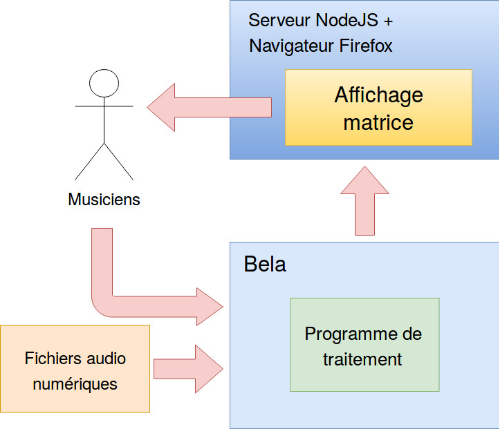
\includegraphics[scale=0.5]{schemaglobal.png}
 \verb!\caption{Schéma global du dispositif de VisualImpro}!
 \label{schéma global}
\end{figure}

\paragraph{}
Ci-dessus, un schéma global du fonctionnement du dispositif. Les
musiciens jouent un morceau traité par Bela qui, via l'intermédiaire
d'une machine, affiche sur le navigateur web Mozilla Firefox la
matrice graphique de corrélations censée assister le jeu des
musiciens.

\paragraph{}
Différentes pistes ont été proposées par Jérémy dans son rapport pour
améliorer le logiciel produit : implémenter un retour sonore indiquant
aux musiciens la qualité des corrélations en fonction du coefficient
calculé à la place du retour visuel, ajouter des effets audio aux
pistes sonores en amont du calcul de corrélation...

\newpage
\section{Analyse des besoins}

\subsection{Besoins fonctionnels}
\paragraph{}
L'objectif principal de notre projet est l'implémentation d'un retour
sonore sur la sortie audio dont dispose le système embarqué. Grâce à
la technologie de Bela, on devrait être en mesure de remplacer ou
compléter le retour visuel par une évaluation audio du jeu des
musiciens.
\paragraph{}
Ce qui motive ce besoin particulier est l'intérêt technologique que
représente l'utilisation de Bela pour produire un résultat sonore
dépendant de nos traitements de calcul mais également de fournir une
assistance aux musiciens supposée plus efficace qu'un simple affichage
visuel. En effet, lorsqu'un groupe tente d'improviser ensemble, il ne
doit pas être évident pour ses membres de se focaliser sur un code
couleur ou un affichage visuel dynamique pour adapter et réviser leurs
jeux. Ce sur quoi se basent usuellement des musiciens tentant de
s'accorder les uns avec les autres sans partition ou chef d'orchestre,
c'est bien évidemment le son, celui que produisent les autres. Avec
l'implémentation de cette sortie sonore, qui serait une version
modifiée en temps réel du morceau joué en entrée du système, on tente
de dénaturer cette logique et d'apporter aux musiciens une nouvelle
façon d'improviser qui, selon les configurations du logiciel choisies,
pourra se révéler plus efficace. Ce nouvel outil mérite quelques
éclaircissements quant à son fonctionnement et son intérêt global.
\paragraph{}
Le retour sonore dont il est question est une version modifiée du
morceau joué en temps réel. Ce morceau est composé du même nombre de
pistes instrumentales que celui interprété en entrée du système
embarqué, mais chacune de ces pistes est préalablement modifiée en
terme de niveau sonore en fonction du coefficient de corrélation. Une
interface de configuration dans le logiciel permettrait alors à
l'utilisateur de définir une "consigne", une loi décrivant quelles
pistes doivent être augmentées en niveau sonore par rapport aux autres
dans le retour et selon quels critères. L'exemple de configuration qui
nous a semblé le plus judicieux est le suivant : les paires de
musiciens les plus corrélées entre elles seront plus augmentées en
niveau sonore dans le morceau de retour. Nous avons imaginé d'autres
configurations possibles : augmenter en niveau sonore les pistes étant
les plus corrélées avec une "piste de référence" ayant pour rôle de
"mener" l'improvisation, augmenter en niveau sonore les paires de
pistes instrumentales les moins corrélées, augmenter en niveau sonore
les pistes dont les sommes des coefficients de corrélation avec toutes
les autres sont les plus élevées...
\paragraph{}
L'intérêt du logiciel a alors légèrement changé, et peut paraître plus
difficile à comprendre. Ce retour sonore, qui pourra être combiné ou
non avec l'affichage visuel de la matrice, a le rôle nouveau de
"provoquer" les musiciens. On les désoriente volontairement, en leur
faisant entendre via des casques auditifs un morceau qui n'est pas
celui qu'ils sont en train de jouer, mais une version différente, où
la musique de chacun est soit augmentée soit diminuée par rapport à
celles des autres en terme de niveau sonore. Cela aura pour
conséquence de motiver les musiciens lésés par ce nouveau mixage à
redoubler d'efforts pour adapter leurs jeux, pour modifier
positivement les couleurs de leurs lignes/colonnes dans la matrice
graphique, afin que le logiciel "approuve" leur performance et
rehausse leur musique dans le mix de sortie.
%SCHEMA GLOBAL LEGEREMENT MODIFIE

\paragraph{}
Comme vous pouvez le constater ci-dessus, le schéma global de
fonctionnement de l'outil n'a pas tellement changé. Cependant, le
changement qu'on apporte a une conséquence indéniable sur le jeu des
musiciens, puisqu'il les désoriente en trompant leur audition et les
force à se concentrer davantage sur la matrice pour comprendre les
rouages du logiciel... et à force de plusieurs utilisations de
celui-ci sous diverses configurations, pour comprendre les rouages de
la notion même d'improvisation.
\paragraph{}
Un autre besoin fonctionnel indispensable est l'implémentation d'une
interface permettant à l'utilisateur de sélectionner ses
configurations ; non seulement les fichiers de
\textit{pre-processing}/calcul de coefficient/calcul de triplet RGB,
mais également la "consigne" déterminant quelles pistes doivent être
augmentées ou diminuées dans le retour sonore.

\subsection{Besoins non fonctionnels}
Au cours de son travail, Jérémy Lixandre a pris soin de rendre
génériques les trois fonctions de \textit{pre-processing}, de calcul
de coefficient de corrélation et de calcul du triplet RGB. Afin de
coller avec l'architecture de Bela et avec ses travaux, nous devrons
tâcher de rendre notre fonction de mixage du retour audio générique
également. De plus, il faudra veiller à ce que son calcul n'entraîne
pas de latence, et que le retour parvienne aux musiciens sans décalage
temporel par rapport à leur jeu.
\paragraph{}
Le refactoring du code est également nécessaire au projet. En effet,
certains choix effectués par notre prédécesseur sur celui-ci nous
paraissent discutables. Notamment, le code est peu commenté, il est
parfois impossible de distinguer le code pré-existant dans Bela de
celui écrit par le programmeur, et le choix des outils destinés à
l'affichage de la matrice nous paraissent discutables. En effet,
Jérémy Lixandre ne semble pas justifier l'emploi de NodeJS et d'un
navigateur web pour l'affichage de la matrice graphique. Nous
choisissons alors de modifier ce processus d'affichage : la matrice
sera affichée via une simple interface graphique du framework Qt, ce
qui nous permet de rassembler l'ensemble du projet sous le langage
C++.
\paragraph{}
Le travail à effectuer sur le code existant se découpe alors en deux
parties : le refactoring du code d'une part, et l'implémentation du
retour sonore d'autre part.

\section{Description détaillée du nouveau logiciel}
\paragraph{}
Nous allons vous présenter la version actuelle du logiciel VisualImpro.

\section{Ajout de fonctionnalités}

\subsection{L'implémentation du retour sonore}
\paragraph{}
Dans le programme de Jérémy Lixandre, la classe \verb!Parser! a pour
utilité de récupérer les informations du fichier de configuration
\verb!config.cfg!, notamment toutes les fonctions de
\textit{processing}. Ce fichier a donc été modifié afin de prendre en
compte notre nouvelle fonction de \textit{processing}, la fonction de
mixage, qui vient s'ajouter aux trois existantes. Tout comme ces
fonctions, elle est générique et doit pouvoir être sélectionnée par
l'utilisateur depuis un menu de configuration.

\paragraph{}
Un fichier dédié à la fonction de mixage a un nom commençant par
\verb!Mix!. Il est répertorié dans le dossier \verb!Mix! du dossier
\verb!Process!. La fonction de mixage doit prendre une matrice en
paramètre ; il s'agit de la matrice retournée par la fonction de
calcul du coefficient de corrélation. Elle retourne un vecteur de
coefficients : à un instant donné, chaque piste dispose désormais d'un
seul coefficient qui doit déterminer la façon dont elle va être
diminuée en volume sonore dans le retour audio.

\paragraph{}
Nous avons implémenté plusieurs fonctions de mixage. La fonction
\verb!vector<float>!
\\ \verb!MixMaxCorrelated!, par
exemple, renvoie un coefficient égal à la moyenne des coefficients de
corrélation de la piste avec toutes les autres pistes. Les instruments
les moins corrélés recevront ici un malus sur l'amplitude de leur signal.
Tandis que la fonction de traduction du coefficient de corrélation en
triplet RGB est dédiée uniquement au retour visuel, celle de mixage est
dédiée uniquement au retour sonore.

\begin{lstlisting}
vector<float> MixMaxCorrelated(const Matrix<float>& correlMatrix) {

  int row = correlMatrix.getSize();
  int col = correlMatrix.getRow(0).size();

  // initialize the result vector with zeros
  vector<float> meanCorrelations(row, 0.0f);

  // fill the vector with the mean correlation of
  // each instrument with others
  for (int i = 0; i < row; i++) {
    for (int j = 0; j < col; j++) {
      if (i != j)
        meanCorrelations[i] += correlMatrix.getCase(i, j);
    }
    meanCorrelations[i] /= (float)row-1;
  }

  return meanCorrelations;
}
\end{lstlisting}

\begin{center}
 \textit{Ci-dessus, l'exemple de la fonction de mixage précédemment cité}
\end{center}

\paragraph{}
Dans la fonction \verb!void parseProcessFunc!  appelée dans le fichier
\verb!main.cpp!, nous avons dû ajouter l'analyse de la fonction de
mixage sur le modèle des analyses des trois autres fonctions de
\textit{processing}.

\paragraph{}
L'architecture de Bela a été conçue pour permettre la synthèse d'un
retour sonore dans le corps de la fonction \verb!void render! du
fichier éponyme. Grâce au code implémenté par notre prédécesseur au
sein de cette fonction, Bela peut synthétiser un retour sonore modifié
par notre fonction de mixage.

\begin{lstlisting}
for(unsigned int i=0; i<context->audioOutChannels; i++){
   if(gSampleFactor == STANDARD_SAMPLE_RATE){
      audioWrite(context, 2 * n, i, out);
      audioWrite(context, 2 * n + 1, i, out);
   } else {
      audioWrite(context, n, i, out);
   }
}
\end{lstlisting}

\begin{center} \textit{Ci-dessus, l'implémentation du retour sonore
  dans le corps de la fonction principale de \verb!render.cpp!. Via la
  fonction \verb!audioWrite!, la variable \verb!out! récupère un à un
  les signaux multipliés par la moyenne de leurs coefficients de
  corrélation par rapport aux autres signaux.} \end{center}

 %  - Ici c'est bien l'écriture du retour sonore, via la variable out, mais ce
 % qui est vraiment important c'est le comportement de la variable out. Elle
 %  récupère les signaux un à un en les additionnant et les stockant dans sa
 %  variable (c'est le cas de base), mais pour notre cas, elle récupère les
 %  signaux multipliés par la moyenne de leur corrélation par rapport aux autres
 %  instruments (valeur comprise entre 0 et 1). On peut voir ça dans les boucles
 %  de chaque type de pistes (audio, analogique ou digitale--pour les fichiers--)%,
 %  pour la boucle de traitement sans effets pour le moment.

 \paragraph{}
 Dans le fichier \verb!render.cpp!, la fonction
 \verb!void processBuffer()! est utilisée comme tâche auxiliaire de la
 boucle de traitement principale. Nous avons déclaré un vecteur
 \verb!gMeanCorrel! dans \verb!render.cpp! ; initialisé avec une valeur
 de 1 pour tous les indices, il prend la valeur que retourne la
 fonction de mixage à l'intérieur du code de la fonction
 \verb!void ProcessMultiCorrel::process!
 que nous avons modifiée et qui est appelée dans \verb!processBuffer!
 de \verb!render.cpp!.
 \paragraph{}
 Dans l'implémentation de Jérémy Lixandre, le traitement des tâches auxiliaires dnas \verb!render.cpp! se faisait à sens unique : exécution de tâches auxiliaires sans retour de valeur dans la boucle de traitement principale. Afin de récupérer le résultat du traitement de la fonction de mixage, nous avons ajouté la référence du vecteur contenant les moyennes de coefficients de corrélation, \verb!gMeanCorrel!, %A FINIR DE REDIGER

 % A expliquer j'ai pas pigé le lien entre gMeanCorrel et process
 - Le traitement des tâches auxiliaires dans le render se faisant à sens
 unique (le render exécute des taches auxiliaires sans renvoyer de valeur de
 retour à la boucle de traitement principale), le moyen pour nous de récupérer
 le résultat du traitement de la fonction de mix était de passer le vecteur
 contenant les moyennes de corrélation, gMeanCorrel, par référence à la
 fonction process. On accède ainsi à la case mémoire de la variable pour
 permettre à la fonction de modifier son contenue et ainsi d'affecter les
 valeurs de retour de la fonction de mixage à notre vecteur. C'est ainsi que
 les modifications des volumes sont possibles dans notre programme.

 \begin{lstlisting}
    void ProcessMultiCorrel::process(const Matrix<float>& buffer,
                                 vector<float>& meanCorrelations,
                                 Connection conn){
  Matrix<float> copy = buffer;

  // Processing functions
  copy = _preprocess(buffer);
  Matrix<float> correlMatrix = calcul_correl(copy);
  process_volume(correlMatrix, meanCorrelations);
  Matrix<RGB> mat = color_matrix(correlMatrix);

  // Send data
  string str = mat.toString();
  conn.send(str);
}
 \end{lstlisting}
 \begin{center}
  \textit{L'appel de la fonction \verb!process! ci-dessus exécute une série de fonctions de traitement de manière séquentielle.}
 \end{center}

 \begin{lstlisting}
    void ProcessMultiCorrel::process_volume(const Matrix<float>&
                                        correlMatrix,
                                        vector<float>&
                                        meanCorrelations){
  meanCorrelations = this->_mixLevel(correlMatrix);
}
  \end{lstlisting}
  \begin{center}
    \textit{Ci-dessus, la fonction appelée dans le corps de la fonction \verb!process!. Nous l'avons implémenté de sorte à altérer en son sein la valeur du vecteur des moyennes de corrélation passé par référence en paramètre.}
  \end{center}

\subsection{L'interface de configuration utilisateur}
\paragraph{}
Afin d'implémenter l'interface de configuration utilisateur précédemment abordée
nous avons ajouté à l'architecture du programme un dossier
\verb!GUI! (\textit{Graphic User Interface}) à la racine du programme.
Le sous-répertoire contenant les fichiers relatifs à l'implémentation de
l'interface de configuration se nomme \verb!settingWindow!.

\begin{figure}[h]
 \centering
 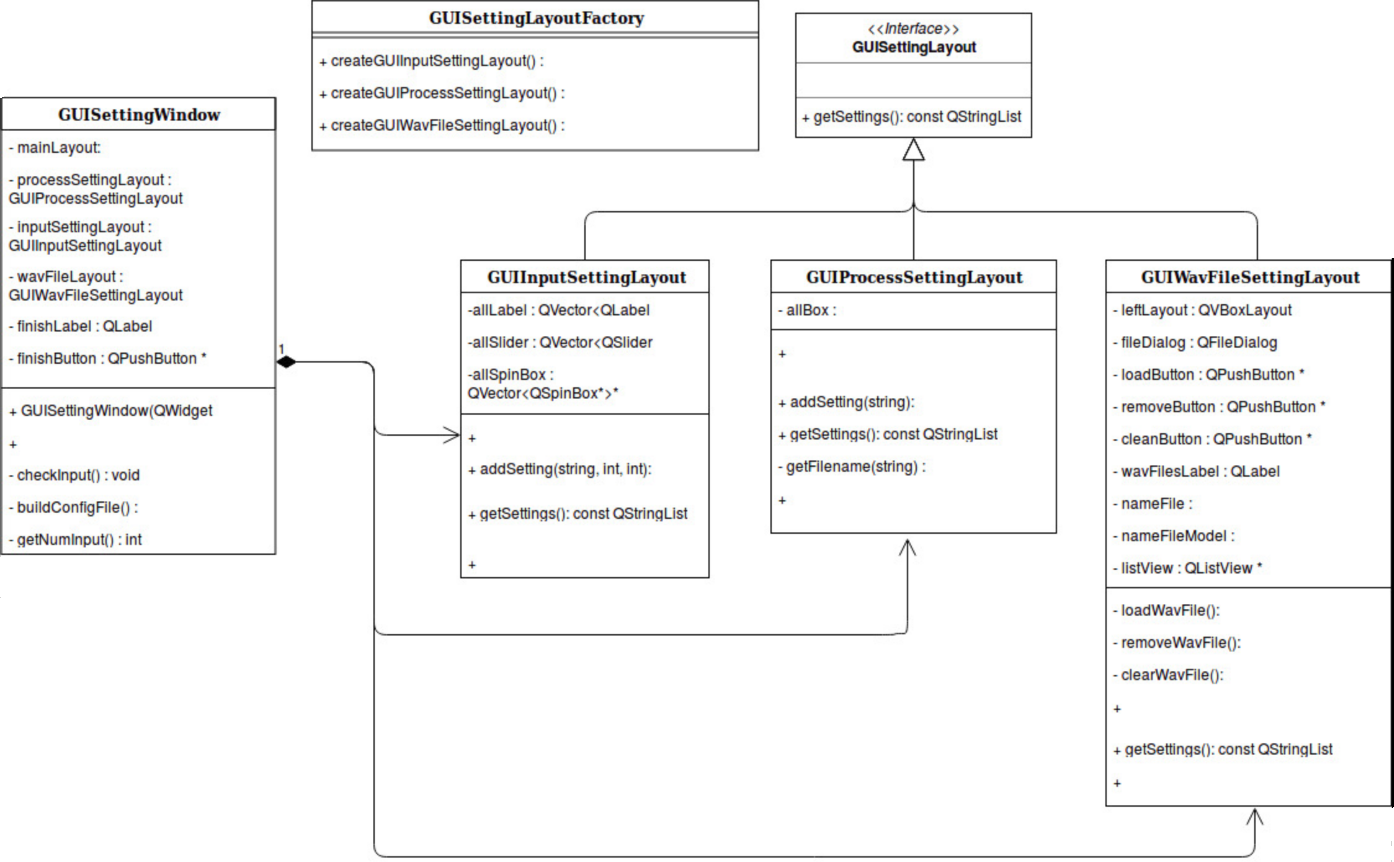
\includegraphics[scale=0.3]{assets/umlSettingWindow.png}
 \caption{Schéma global du dispositif de VisualImpro}
 \label{schéma global}
\end{figure}

\paragraph{}
La classe principale de cette interface de configuration est la
classe \verb!settingWindow!. Elle constitue une fenêtre vide
destinée à afficher les données suivantes :
\begin{itemize}
 \item Paramètres de fonction de traitement.
 \item Paramètres du nombre d'entrées audio et analog.
 \item Choix des fichiers audio \textit{.wav}.
\end{itemize}
En plus de toutes ces parties, la fenêtre principale possède (check la doc)

\begin{figure}[h]
 \centering
 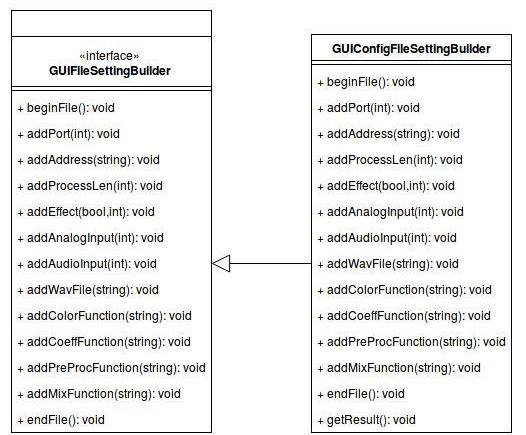
\includegraphics[scale=0.5]{assets/umlBuilder.png}
 \caption{Schéma global du dispositif de VisualImpro}
 \label{schéma global}
\end{figure}

\paragraph{}
La fenêtre de configuration%AJOUTER

\subsection{Autres ajouts mineurs sur le programme}
\paragraph{}
Nous avons implémenté une nouvelle fonction de corrélation dédiée aux
tests : appelée \verb!CoeffRandom!, elle établit un coefficient de
corrélation de manière aléatoire. La généricité de l'implémentation
existante a rendu la tâche triviale, il nous a suffi d'écrire un
fichier d'en-tête \verb!CoeffRandom.hpp! et un fichier source
\verb!CoeffRandom.cpp! dans le dossier \verb!Coeff! contenant les
fonctions de calcul du coefficient de corrélation (dossier
\verb!process!). Cette fonction renvoie un flottant compris entre 0 et
1, comme les autres fonctions de corrélation. L'accomplissement de
cette tâche et la trivialité qu'il représente témoigne de la
généricité des fonctions de corrélation, et des fonctions de
traitement en général, qui possèdent désormais toutes plusieurs
versions alternatives.

\section{Refactoring et révision de l'interface graphique}

\subsection{Révisions générales sur le code}
\paragraph{}
Nous avons rapidement établi que le refactoring du code existant
faisait partie des besoins de notre projet. Dans cette partie, nous
décrirons l'ensemble des travaux réalisés dans ce cadre.

\subsubsection{Conventions de programmation et assistance au programmeur}
\paragraph{}
L'un des premiers reproches faits par l'équipe pédagogique à
l'architecture héritée de Jérémy Lixandre est son manque de clarté ;
le code livré était trop peu commenté pour permettre à un programmeur
de comprendre ne serait-ce que le rôle de chaque classe sans rentrer
en détail dans l'intégralité de leur code. Pour cette raison, nous
avons abondemment commenté le code en rajoutant également de la documentation
doxygen. Pour tous les fichiers sources, nous trouvons dans l'en-tête de chaque
début de fichier \verb!.cpp! le rôle et le fonctionnement de ceux-là.
\paragraph{}
Des commentaires ont également été ajoutés massivement au niveau des
fonctions principales du programme. En effet, la compréhension du
programme existant a considérablement ralenti le démarrage de notre
implémentation sur ce projet, et a nécessité plusieurs recherches sur
le web et la consultation conjointe de divers documents de sources
différentes. Les deux fichiers ayant été les plus commentés de la
sorte sont \verb!main.cpp! et \verb!render.cpp!.
\paragraph{}
La syntaxe du code a été remodelée de manière générale pour répondre à
des conventions autant que pour faciliter sa compréhension : les
"include" en début de fichiers ont été classés selon le type de
fichiers inclus et par ordre alphabétique, la langue des commentaires
a été uniformisée, les indentations, choix de placement de
crochets/accolades etc. ont été uniformisés également pour une
meilleure cohérence de la syntaxe, les variables ont été renommées
pour être plus claires et éviter de heurter les conventions qui nous
ont été enseignées.

\subsubsection{Modification de l'architecture logicielle}
\paragraph{}
D'autres approches du code réalisées par Jérémy Lixandre nous
semblaient maladroites. Afin de rendre une architecture répondant au
mieux aux conventions de programmation vues en cours et qui soit la
plus compréhensible et claire possible aux yeux d'un potentiel futur
programmeur, nous avons apporté plusieurs révisions liées à
l'organisation des fichiers.
\begin{itemize}
  \item Le code de \verb!main.cpp! a été entièrement révisé. En effet,
    il contenait une unique fonction
    \verb!main(int argc, char *argv[])! qui nous paraissait bien trop
    dense. Afin de faciliter la compréhension du lecteur et de mieux
    correspondre aux conventions, nous avons effectué un découpage
    fonctionnel de cette fonction en plusieurs fonctions. La fonction
    \verb!main! appelle une fonction
    \verb!launch(int argc, char *argv[])! qui elle-même appelle
    d'autres fonctions (lesquelles, parfois, en appellent elles-mêmes
    de nouvelles).

    \begin{lstlisting}
      static void launch(int argc, char *argv[]){
        ChSettings gChSettings;
        Parser config;
        void *handle;
        ProcessMultiCorrel *p;
        config = initParser(argc, argv);
        handle = initHandler();
        p = initProcessMultiCorrel(handle);
        setupSettings(gChSettings, config, p, handle);
        initAndRun(gChSettings, config, argv);
        stopAndCleanupAudio();
        freeAndClose(gChSettings, config, p, handle);
      }
    \end{lstlisting}

    \begin{center}
      \textit{Ci-dessus, le code de la fonction launch}
    \end{center}

    \item Nous avons de même effectué un découpage fonctionnel sur la
      fonction \\ \verb!bool setup!  du fichier \verb!render.cpp!. Ce
      fichier, qui présentait tout comme \verb!main.cpp! une
      organisation assez condensée, ne pouvait pas cependant être
      remanié autant en profondeur dans son intégralité que le code
      précédemment abordé. En effet, la fonction principale du
      fichier, \verb!void!  \verb!render!, ne pouvait être découpée de
      manière maintenable. En effet, elle exécute une boucle de
      traitement audio, en créant des taches auxiliaires exécutées par
      d'autres threads pour garantir un traitement rapide (qui doit
      être au minimum plus rapide que la vitesse de lecture des
      pistes), et il n'était pas possible de la découper sans créer de
      conflits sur les variables enregistrant le nombre de tours de
      boucle ou les variables contenant les signaux audio par exemple.

      \begin{lstlisting}
      bool setup(BelaContext *context, void *userData) {
        gUserSet = *((ChSettings *)userData);
        initUserSet(gUserSet);
        initBuffers();
        initSampleStreams(gUserSet);
        printInfo();
        return initAuxiliaryTasks();
      }
    \end{lstlisting}

    \begin{center}
      \textit{Ci-dessus, le code de la fonction setup}
    \end{center}

      \item \`{A} l'intérieur du dossier \verb!process!, les
        différents fichiers de traitement ont été classés par
        fonctions en quatre dossiers \verb!Coeff!, \verb!Color!,
        \verb!Preproc! et \verb!Mix!. \`{A} l'intérieur du dossier
        \verb!test!, les fichiers que nous avons implémenté pour tester les
        différentes fonctions du programme ont été classés de la même
        manière (Jérémy Lixandre n'avait pour sa part pas implémenté
        de fichiers de test). Le fichier TestMain contenu à la racine du
        dossier test se chargera de récupérer le registre de l'ensemble
        des tests contenus dans les différents dossiers.

        \item D'une manière générale, les fichiers ont été triés pour
          ordonner l'architecture proposée par Jérémy qui était un peu
          confuse ; des fichiers de code n'ayant rien à voir entre eux
          se côtoyaient au sein d'un même dossier, et l'architecture
          présentait une hiérarchie n'étant pas toujours en rapport
          avec celle que présente le logiciel. Pour ces raisons, nous
          avons partagé les fichiers en plusieurs sous-dossiers,
          notamment les fichiers sources et les fichiers d'en-tête au
          sein du dossier \verb!VisualImpro!, et nous avons modifié
          les fichiers Makefile en conséquence. Le fichier de
          configuration \verb!config.cfg! a notamment été déplacé dans
          un nouveau dossier \verb!bin!.

          \item Dans le code livré par Jérémy Lixandre, un dossier
            \verb!VisualImproExe! regroupait un fichier de
            configurations, les fichiers relatifs à NodeJS, un fichier
            html lié à l'affichage de la matrice graphique via le
            navigateur Mozilla Firefox et les fichiers sources C++
            permettant les manipulations nécessaires au lancement du
            programme VisualImpro. Nous avons implémenté un script
            bash voué à remplacer la majeure partie de cette
            architecture, le fichier \verb!VisualImpro.sh! placé dans
            le dossier \verb!bin!.
\end{itemize}
\paragraph{}
Dans la version précédente de l'exécutable (\verb!VisualImproExe!),
les tâches réalisées par le code C++ étaient les suivantes :
\begin{itemize}
  \item Copier les fichiers \verb!.wav! indiqués dans le fichier de
    configuration dans Bela,
  \item Créer une copie du fichier de configuration, et y modifier les
    chemins des fichiers \verb!.wav! pour que ceux-ci correspondent au
    système de fichiers de Bela,
  \item Copier la copie du fichier de configuration dans Bela,
  \item Lancement du serveur NodeJS avec le fichier \verb!server.js!,
  \item Ouverture d'un onglet (ou d'une nouvelle fenêtre) du
    navigateur Firefox,
  \item Connexion à Bela (en ssh) et lancement du programme
    VisualImpro,
  \item Si le programme reçoit un signal d'interruption (Ctrl-C),
    alors certaines tâches sont réalisées :
  \begin{itemize}
    \item Arrêt du programme VisualImpro,
    \item Arrêt du serveur NodeJS,
    \item Suppression des fichiers \verb!.wav! sur Bela,
    \item Rapatriement des logs vers le dossier \verb!VisualImproExe!,
    \item Suppression de la copie modifiée du fichier de configuration,
    \item Arrêt de l'éxécutable.
  \end{itemize}
\end{itemize}
\paragraph{}
Durant l'audit, le fait de réaliser des manipulations de fichiers de
configuration, ainsi que des transferts de fichiers ou des connexions
vers Bela à l'aide de fichiers C++ a été pointé du doigt. En effet,
cette façon de faire reposait sur des classes C++ annexes qui
effectuaient les manipulations de chaînes de caractères dans les
fichiers de configuration, et pour ce qui concerne le transfert de
fichiers et la connexion vers Bela, cela été réalisé à l'aide d'appels
à la fonction C \verb!int system(const char *command)!.
\paragraph{}
Réaliser toutes ces opérations à l'aide d'un script bash paraissait
beaucoup plus pertinent. Cela permet de se passer des différents
fichiers sources et d'en-tête C++, et de plus, il existe des commandes
bash permettant de réaliser ces manipulations de chaînes de caractères
de façon beaucoup moins lourde et fastidieuse.
\paragraph{}
En plus de reproduire le comportement de l'ancienne version de
l'exécutable, notre script bash \verb!VisualImpro.sh! permet de
choisir entre les deux versions graphiques maintenant disponibles. Il
suffit de préciser à l'aide d'une option (\verb!qt! ou \verb!firefox!)
quel affichage on souhaite obtenir.
\paragraph{}
Parmi les autres aspects de l'existant que nous avons tenu à réviser,
la classe utilities posait problème dans le sens où elle contenait un
trop grand nombre de fonctions n'ayant rien à voir entre elles. Nous
avons tâché de réduire son contenu au maximum, et actuellement, elle
ne contient plus que deux fonctions utilisées par les fichiers
\verb!main.cpp! et \verb!render.cpp!, et son rôle est véritablement
celui d'une classe utilitaire pour les fichiers principaux du
programme.

- La classe utilities contenait un trop grand nombre de fonctions et était
  utilisée comme la classe "fourre-tout" à inclure partout. On a donc réduit
  au maximum son contenu pour qu'elle contienne le minimum de fonctions
  possibles. Elle contient actuellement seulement 2 fonctions utilisées par le
  main et le render, et joue vraiment le rôle de classe utilitaire pour les
  fichiers principaux de notre programme. Pour la réduire au maximum, il fallait
  dans un premier temps supprimmer les fonctions de traitement qu'elle contenait
  (et qui faisait que cette classe devait être incluse dans tous les fichiers du
  répertoire process), et les placer dans le code de manière stratégique pour
  éviter cette inclusion systématique, et d'autre part il fallait
  supprimer la structure Triplet qu'elle contenait, qui correspondait à un
  triplet RGB, et nous avons créé une classe RGB en conséquence. Elle regroupe
  les fonctions utilisées pour la classe triplet, refactorées pour la cette
  nouvelle classe RGB en améliorant le code des fonctions initiales. Les
  fonctions créées par le stagiaires pour passer d'entiers vers des valeurs
  hexadecimales ont été refactorées de manière à les rendre plus simples tout
  en gardant le même résultat en sortie.

\subsubsection{Optimisation du code}
\paragraph{}
Afin de garantir un traitement rapide des informations par BELA et de
produire un retour sonore sans risque de latence, nous avons dû
optimiser certaines parties du code. Dans son rapport, Jérémy Lixandre
avait précisé que le traitement de BELA occupait une part trop
importante du CPU à partir de quinze fichiers \verb!.wav! traités
simultanément ; ce constat nous a encouragés à optimiser le programme
pour limiter le coût de son exécution.
\paragraph{}
L'implémentation de l'existant présentait notamment de nombreuses
copies des matrices passées en paramètres. Ces matrices sont des
éléments particulièrement lourds, contenant un nombre de données égal
au produit du nombre de pistes sonores en entrée par 32768 (taille des
buffers traités). Nous avons choisi de remplacer ces copies
successives de matrices par le placement en paramètres de références
constantes de ces matrices.

\begin{lstlisting}
void ProcessMultiCorrel::process(const Matrix<float>& buffer,
                                 vector<float>& meanCorrelations,
                                 Connection conn){
  Matrix<float> copy = buffer;

  // Processing functions
  copy = _preprocess(buffer);
  Matrix<float> correlMatrix = calcul_correl(copy);
  process_volume(correlMatrix, meanCorrelations);
  Matrix<RGB> mat = color_matrix(correlMatrix);

  // Send data
  string str = mat.toString();
  conn.send(str);
}
\end{lstlisting}
\begin{center}
  \textit{Ci-dessus, la fonction principale de
    \verb!ProcessMultiCorrel.cpp!. Ce code témoigne de multiples
    opérations de refactoring et d'optimisations du code ; en effet,
    le nombre d'appels de fonctions au sein de la fonction process témoigne du
    découpage fonctionnel de la fonction d'origine, laquelle était autrement
    plus dense. De plus, on peut observer dans les paramètres qu'un
    vecteur des moyennes de coefficients de corrélation a été ajoutée
    pour permettre l'implémentation du mixage du retour sonore. Enfin,
    la matrice de flottants "buffer" a été changée en sa référence
    constante, afin d'éviter d'avoir à en faire une copie dans le
    corps de la fonction.}
  \end{center}

% A AJOUTER
\subsubsection{Autres remarques}
  

  - Nous avions beaucoup de traitements sur des matrices dans notre code, mais
  nous ne disposions auparavant pas de classe pour répondre à ce besoin, ce qui
  faisait que nous utilisions des vecteurs de vecteurs de flottants pour nos
  traitements. Cela était très lourd d'écriture, et demandait d'écrire des
  fonctions de traitement de vecteurs de vecteurs quelque part pour nos
  opérations, et ces fonctions étaient donc définies dans le fichier utilities
  avec le reste. Nous avons donc créé une classe Matrix correspondant à un
  vecteur de vecteur et contenant toutes les opérations sur les matrices dont
  nous avons besoins, en plus de nombreux constructeurs pour créer des matrices
  de différents types, selon différents paramètres. Cette classe Matrix est une
  classe template, et permet ici de créer des matrices d'entiers, de flottants,
  ou bien de triplets RGB.

  -Nous avons effectué des tests de ces deux nouvelles classes, Matrix et RGB,
  dans le dossier de TestClasses lui même dans le dossier test, contenant
  l'ensemble des dossiers de tests regroupés par cohérence de type.

  - Les classes ProcessMultiCorrel et ProcessMultiWriteWav héritaient d'une
  classe nommée ProcessMulti, mais l'héritage ici n'avait pas lieu d'être car
  cette classe ProcessMulti définissait une fonction abstraite process,
  redéfinie dans ses classes filles, et prenant en paramètre une matrice de
  flottants (signaux) et une connexion. Or la classe ProcessMultiWriteWav sert
  à créer des fichiers .wav, donc ne requiert aucune connexion. Ce paramètre
  n'était donc pas utilisé dans la fonction process de la classe
  ProcessMultiWriteWav, et comme l'on devait rajouter un paramètre pour notre
  fonction process de la classe ProcessMultiCorrel, l'héritage n'était
  clairement plus justifié. Nous avons donc cassé l'héritage entre ces classes
  et supprimé la classe ProcessMulti.

  - Ajout de fichiers header pour tous les fichiers source contenant les
  fonctions de traitement. Cela permet de pouvoir utiliser chaque fonction en
  incluant le fichier contenant la fonction dont nous avons besoin. Auparavant,
  nous copions chaque fonction de traitement (ou du moins des parties "utiles"
  des fonctions de traitement) dans la classe utilities, mais cette dernière
  ayant été réusinée de manière à être cohérente et non un gros sac ignoble,
  nous devons donc coder proprement et inclure le fichier header de la fonction
  que nous voulons utiliser, comme par exemple pour nos fichiers de test.
%A AJOUTER

\subsection{Les changements apportés à l'interface graphique}
\paragraph{}
Précédemment, nous parlions de la nécessité de modifier l'affichage de
l'interface graphique pour diverses raisons. Nos clients n'exprimaient
pas de préférence quant à la méthode employée pour afficher la matrice
imaginée par nos prédécesseurs de l'ENSEIRB, mais nous trouvions peu
judicieux et coûteux pour le programme de passer par NodeJS et Mozilla
Firefox pour la produire. Un affichage graphique implémenté en C++
grâce au framework Qt nous paraissait plus logique, judicieux et
conforme au reste de l'architecture de notre programme.
\paragraph{}
Cependant, nous pouvons reconnaître l'avantage que peut avoir
l'affichage de la matrice sur un navigateur répandu comme Mozilla
Firefox. En effet, on peut imaginer qu'à l'avenir, le programme
embarqué sur le système Bela pourra se passer d'un ordinateur pour
fonctionner et afficher la matrice sur l'écran d'un smartphone par
exemple en passant par un navigateur web. Pour cette raison, nous
avons décidé d'offrir à l'utilisateur la possibilité de choisir entre
l'affichage Qt et l'affichage sur navigateur au moment de lancer
l'exécution du programme.

\subsubsection{L'implémentation de la méthode d'affichage sous Qt}

\newpage
\section{Tests du logiciel}

\subsection{Tests unitaires}

\paragraph{}
Les tests, absents de la version du logiciel VisualImpro livrée par
Jérémy Lixandre, ont été entièrement implémentés par nos soins. Nous
les avons regroupés dans un dossier \verb!Tests! qui comprend un
fichier source \verb!TestMain.cpp!, lequel affiche les résultats de
tous les autres fichiers de test sur la sortie standard, et six
répertoires contenant ces fichiers de test. Il contient également un
\verb!Makefile! et un répertoire \verb!Sine-samples! contenant des
signaux sinusoïdaux à tester.

\subsubsection{Tests de classes}
\paragraph{}
Le répertoire \verb!TestClasses! vérifie le bon fonctionnement de
certaines classes.

\paragraph{}
Le fichier \verb!TestMatrix.cpp! est implémenté dans le but de
démontrer le correct fonctionnement de la classe codant l'objet
matrice, de la classe \verb!Matrix.cpp!. Il teste des opérations
portant sur des matrices, sur des cases, des lignes et des colonnes
spécifiques de matrices.

\paragraph{}
Le fichier \verb!TestMultiCorrel.cpp! teste des opérations de base sur
l'objet permettant de traiter le retour sonore,
\verb!ProcessMultiCorrel.cpp!, telles que des opérations d'accès et
d'écriture basiques \textit{getter/setter} aux données membres de la
classe.

\subsubsection{Tests de la fonction de traduction du coefficient de corrélation en triplets RGB}
\paragraph{}
Le répertoire \verb!TestColor! contient deux fichiers de test testant
chacun le bon fonctionnement des deux fonctions de traduction du
coefficient de corrélation en triplet RGB (la première établit un code
couleur allant du rouge au vert, la seconde un code couleur en niveaux
de gris allant du noir au blanc). Ces tests fonctionnent en vérifiant
que des flottants ayant des valeurs extrêmes et une valeur
intermédiaire retournent bien les couleurs attendues, par exemple :
une couleur rouge pour un coefficient de 0 avec la première fonction.

\subsubsection{Tests de la fonction de pré-traitement}
\paragraph{}
Le répertoire \verb!TestPreproc! contient trois fichiers de test, un
pour chacune des trois fonctions de pré-traitement
existantes. L'implémentation de \verb!TestPreprocDefault.cpp!,
\verb!TestPreprocEnergy.cpp! et \verb!TestPreprocStrenghtEnergy.cpp!
permet de comparer le résultat des fonctions de pré-traitement
correspondantes, prenant des matrices simples en paramètres, avec les
résultats attendus.

\subsubsection{Tests de la fonction de calcul de coefficient de corrélation}
\paragraph{}
Le répertoire \verb!TestCoeff! contient deux fichiers testant chacun
l'une de nos deux fonctions de calcul de coefficient de
corrélation. Le premier, \verb!TestCoeffScalar.cpp!, vérifie que la
fonction testée renvoie bien la bonne valeur en comparant son résultat
pour deux vecteurs arbitraires passés en paramètre avec le résutat du
calcul brut du produit scalaire de ces deux mêmes vecteurs, qui
doivent être égaux. Le second fichier de test unitaire,
\verb!TestCoeffRandom!, teste que pour mille itérations, le résultat
de la fonction testée est toujours compris dans l'ensemble de valeur
attendu (entre 0 et 1).

\subsubsection{Tests de la fonction de mixage}
\paragraph{}
Les fichiers contenus dans le répertoire \verb!TestMix! s'assurent
pour chaque fonction de mixage existante que le résultat obtenu pour
une matrice passée en paramètre de la fonction est égal à celui
attendu. Par exemple, la fonction de \verb!MixNeutral.cpp!, qui simule
l'absence de fonction de mixage, doit renvoyer 1 comme coefficient de
modification du volume sonore quelque soit la matrice d'entrée ; on
s'en assure dans le fichier de test \verb!TestMixNeutral.cpp!.

\subsubsection{Test de l'interface graphique utilisateur}
Les fichiers contenus dans le répertoire \verb!TestGUI! assurent
le fonctionnement de l'interface graphique. Le seul test implémenté
et le test du builder qui est la seule classe qui construit le fichier description
de configuration.
En effet, hormis en utilisant une capture d'écran de l'affichage voulu afin
de la comparer à celle qui est affichée, il est difficile de tester
une interface graphique.

\subsection{Test globaux}
\paragraph{}
Pour tester l'outil dans son intégralité, i lfallait des échantillons pour lesquels nous connaissions les résultats à l'avance. Pour cela, nous avons généré des signaux sinusoïdaux et carrés, car ce sont les signaux les plus simples. Nous en avons généré plusieurs, et à chaque fois, nous avons décalé les phases pour pouvoir réaliser plusieurs tests. De plus, nous avons réalisé nos tests avec deux focntions de pré-traitement différentes : \verb!PreprocDefault! et \verb!PreprocStrengthEnergy!. La première ne touche pas au signal, la seconde transforme la composante négative en positive.
\subsubsection{Avec PreprocDefault}
\paragraph{}
Les figures suivantes doivent être interprétées de la façon suivante : plus la couleur est verte, plus les signaux sont proches, plus on tend vers le rouge, plus les signaux sont différents.
\begin{figure}[H]
    \centering
    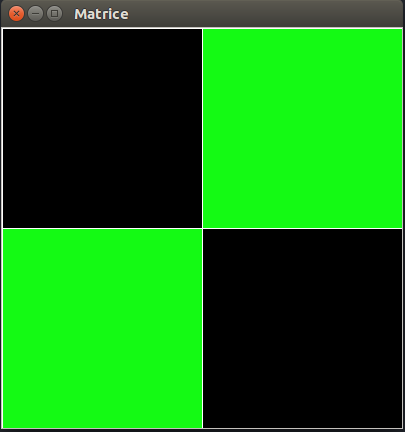
\includegraphics[scale=0.3]{assets/Captures-sinus/PreprocDefaultnormal-normal.png}
    \caption{Test avec deux sinus identiques}
    \label{}
\end{figure}
\begin{figure}[H]
    \centering
    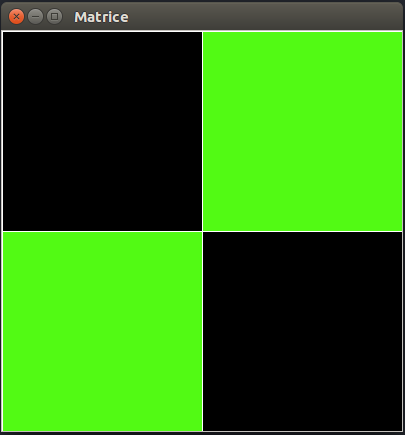
\includegraphics[scale=0.3]{assets/Captures-sinus/PreprocDefaultnormal-30.png}
    \caption{Test avec deux sinus décalés de 30 degrés}
    \label{}
\end{figure}
\begin{figure}[H]
    \centering
    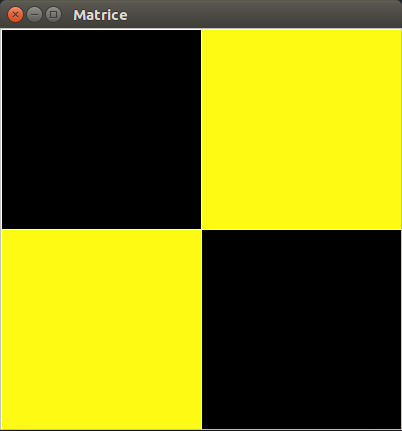
\includegraphics[scale=0.3]{assets/Captures-sinus/PreprocDefaultnormal-60.png}
    \caption{Test avec deux sinus décalés de 60 degrés}
    \label{}
\end{figure}
\begin{figure}[H]
    \centering
    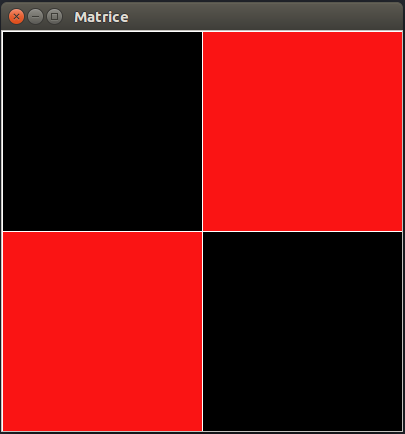
\includegraphics[scale=0.3]{assets/Captures-sinus/PreprocDefaultnormal-90.png}
    \caption{Test avec deux sinus décalés de 90 degrés}
    \label{}
\end{figure}
\paragraph{}
À 90 degrés, les sinus sont inversées, d'où le fait que la corrélation soit nulle.
\begin{figure}[H]
    \centering
    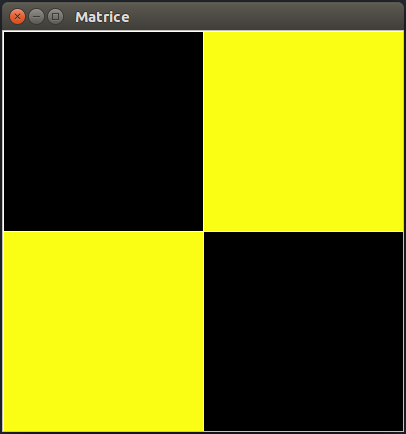
\includegraphics[scale=0.3]{assets/Captures-sinus/PreprocDefaultnormal-120.png}
    \caption{Test avec deux sinus décalés de 120 degrés}
    \label{}
\end{figure}
\begin{figure}[H]
    \centering
    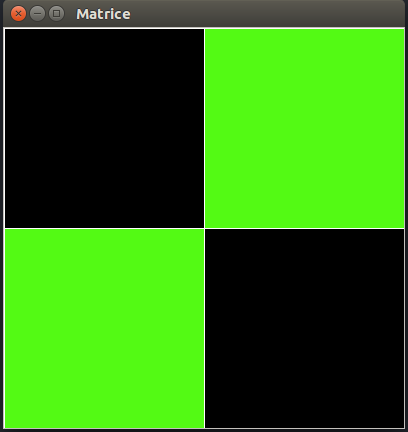
\includegraphics[scale=0.3]{assets/Captures-sinus/PreprocDefaultnormal-150.png}
    \caption{Test avec deux sinus décalés de 150 degrés}
    \label{}
\end{figure}
\begin{figure}[H]
    \centering
    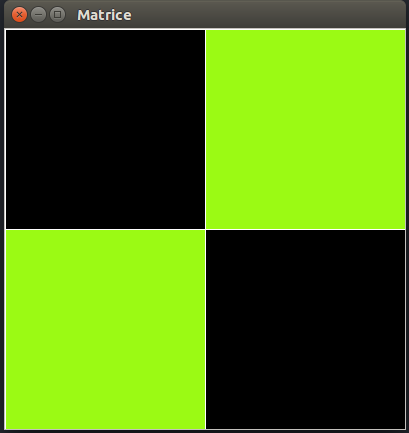
\includegraphics[scale=0.3]{assets/Captures-sinus/PreprocDefautnormal-180.png}
    \caption{Test avec deux sinus décalés de 180 degrés}
    \label{}
\end{figure}
\subsubsection{Avec PreprocStrenghtEnergy}
\begin{figure}[H]
    \centering
    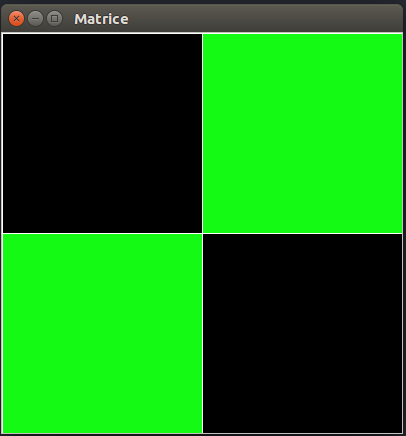
\includegraphics[scale=0.3]{assets/Captures-sinus/PreprocStrengthnormal-normal.png}
    \caption{Test avec deux sinus identiques}
    \label{}
\end{figure}
\begin{figure}[H]
    \centering
    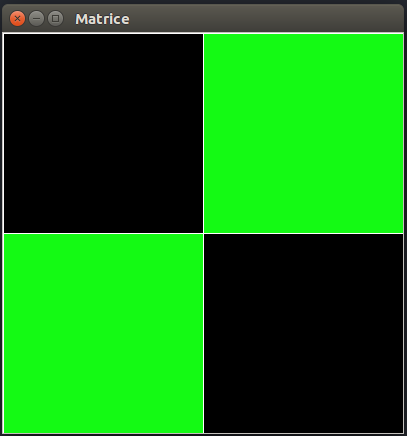
\includegraphics[scale=0.3]{assets/Captures-sinus/PreprocStrengthnormal-90.png}
    \caption{Test avec deux sinus décalés de 90 degrés}
    \label{}
\end{figure}
\paragraph{}
Avec PreprocStrenghtEnergy, comme il n'y a plus de valeurs négatives, la sinus décalée de 90 degrés est identique à la sinus normale.
\begin{figure}[H]
    \centering
    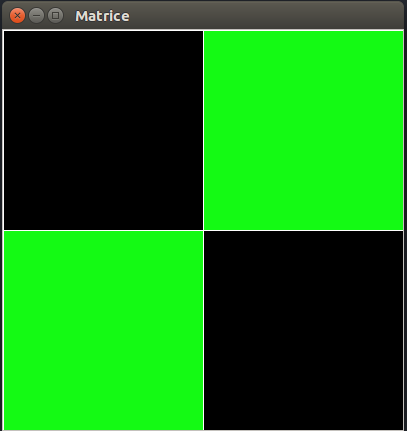
\includegraphics[scale=0.3]{assets/Captures-sinus/PreprocStrenghtnormal-180.png}
    \caption{Test avec deux sinus décalés de 180 degrés}
    \label{}
\end{figure}
\section{Conclusion}
      %A faire

\bibliography{memoire}
\end{document}
